%% The following macros taken from the CMS note
\renewcommand{\gg}{\ensuremath{\PGg\PGg}\xspace}
\newcommand{\hgg}{\ensuremath{\PH\to\gg}\xspace}
\newcommand{\ggh}{\ensuremath{\Pg\Pg\PH}\xspace}
\newcommand{\vbf}{\ensuremath{\mathrm{VBF}}\xspace}
\newcommand{\vh}{\ensuremath{\mathrm{V}\PH}\xspace}
\newcommand{\tth}{\ensuremath{\Pqt\Pqt\PH}\xspace}
\newcommand{\zz}{\ensuremath{\PZ\PZ}\xspace}
\newcommand{\hzz}{\ensuremath{\PH\to\zz}\xspace}
\newcommand{\hzzllll}{\ensuremath{\hzz^{(\ast)}\to 4\ell}\xspace}
\newcommand{\ww}{\ensuremath{\PW\PW}\xspace}
\newcommand{\hww}{\ensuremath{\PH\to\ww}\xspace}
\newcommand{\hwwlnln}{\ensuremath{\hww^{(\ast)}\to\ell\Pgn\ell\Pgn}\xspace}
\newcommand{\bb}{\ensuremath{\PQb\PQb}\xspace}
\newcommand{\hbb}{\ensuremath{\PH\to\bb}\xspace}
\newcommand{\tautau}{\ensuremath{\Pgt\Pgt}\xspace}
\newcommand{\htt}{\ensuremath{\PH\to\tautau}\xspace}
\newcommand{\hlep}{\ensuremath{\PH\to\text{leptons}}\xspace}
\newcommand{\mumu}{\ensuremath{\PGm\PGm}\xspace}
\newcommand{\hmm}{\ensuremath{\PH\to\mumu}\xspace}
\newcommand{\wh}{\ensuremath{\PW\PH}\xspace}
\newcommand{\zh}{\ensuremath{\PZ\PH}\xspace}
\providecommand{\fbinv}{\mbox{\ensuremath{\,\text{fb}^\text{$-$1}}}\xspace}
\newcommand{\SM}{\ensuremath{\mathrm{SM}}\xspace}
\newcommand{\kZ}{\ensuremath{\kappa_{\mathrm{\PZ}}}\xspace}
\newcommand{\kW}{\ensuremath{\kappa_{\mathrm{\PW}}}\xspace}
\newcommand{\ktau}{\ensuremath{\kappa_{\PGt}}\xspace}
\newcommand{\ktop}{\ensuremath{\kappa_{\Pqt}}\xspace}
\newcommand{\kb}{\ensuremath{\kappa_{\Pqb}}\xspace}
\newcommand{\kmu}{\ensuremath{\kappa_{\Pgm}}\xspace}
\newcommand{\kglu}{\ensuremath{\kappa_{\mathrm{\Pg}}}\xspace}
\newcommand{\kgam}{\ensuremath{\kappa_{\PGg}}\xspace}
\newcommand{\GammaSM}{\ensuremath{\Gamma_{\PH}/\Gamma_{\PH}^{\mathrm{SM}}}\xspace}
\newcommand{\Bbsm}{\ensuremath{\mathrm{B_{BSM}}}\xspace}
\newcommand{\kV}{\ensuremath{\kappa_{\mathrm{V}}}\xspace}
\providecommand{\wip}[1]{\textcolor{red}{\bfseries TODO: #1}\xspace}


%% List of input analyses in CMS, add ATLAS too
\wip{Text to be updated to reflect ATLAS+CMS combination.}

The projections documented in this section are based on extrapolations of the following analyses:

\begin{itemize}
	\item \hgg, with $\ggh$, $\vbf$, $\vh$ and $\tth$ production~\cite{Sirunyan:2018ouh},
	\item \hzzllll, with $\ggh$, $\vbf$, $\vh$ and $\tth$ production~\cite{HIG16041},
	\item \hwwlnln, with $\ggh$, $\vbf$ and $\vh$ production~\cite{HIG-16-042},
	\item \htt, with $\ggh$ and $\vbf$ production~\cite{HIG16043},
	\item \vh production with \hbb decay~\cite{HIG16044},
	\item Boosted H production with \hbb~ decay~\cite{HIG17010},
	\item \tth production with \hlep~\cite{Sirunyan:2018shy},
	\item \tth production with \hbb~\cite{bib:hig-17-026,Sirunyan:2018ygk},
	\item \hmm, with $\ggh$ and $\vbf$ production~\cite{HIG-17-019}.
\end{itemize}

The projected results given in this section are based on the combined measurement of these channels~\cite{Sirunyan:2018koj}. In the following results he signal model in the $\hmm$ channel is modified to account for the improved dimuon mass resolution in the Phase-2 CMS tracker upgrade~\cite{Klein:2017nke}. It is estimated that the reduced material budget and improved spatial resolution of the upgraded tracker will yield a $40\%$ improvement in the relative di-muon mass resolution, for example a reduction from $1.1\%$ to $0.65\%$ for muons in the barrel region.

% The results in this section are presented under the two systematic uncertainty scenarios S1 and S2 as described in Section~\ref{sec:extrap}.

\wip{Switch to cross section and branching ratio results without inclusive theory uncertainties.}
Projections are given for two parametrisations of the signal, based on signal strength modifiers $\mu$, defined as the ratio between the measured Higgs boson yield and its SM expectation. One set of parameters $\mu^{f}$, where $f = \zz$, $\ww$, $\gg$, $\tautau$, $\bb$ and $\mumu$, are introduced to scale the branching fractions of each decay mode independently, assuming the SM cross sections for the production modes. Another set, $\mu_{i}$, where $i=\ggh$, $\vbf$, $\wh$, $\zh$ and $\tth$, scale each production cross section independently, assuming the SM values of the branching fractions.

\subsubsection{Signal strength per-decay mode}

The expected $\pm 1\sigma$ uncertainties on the per-decay-mode signal strength parameters in S1 and S2 are summarised in Figure~\ref{fig:summary_A1_5D} with numerical values given in Table~\ref{tab:summary_A1_5D}. The table additionally gives the breakdown of the uncertainty into four components: statistical, signal theory, background theory and experimental. The S2 uncertainties range from $3$--$4\%$, with the exception of that on $\mu^{\mu\mu}$ at $10\%$. The S1 uncertainties are up to a factor of 1.5 larger than those in S2, reflecting the larger systematic component. The dominant uncertainty contribution is found to vary with the scenario and the integrated luminosity of the projection. The systematic uncertainties generally dominate in both S1 and S2. In S2 the signal theory uncertainty is the largest, or joint-largest, component for all parameters except $\mu^{\mu\mu}$, which remains limited by statistics due to the small $\hmm$ branching fraction. The $\mu^{\mu\mu}$ uncertainty using the Run~2 dimuon mass resolution instead of the Phase-2 expectation is $14\%$.


\begin{figure}[hbtp]
\centering
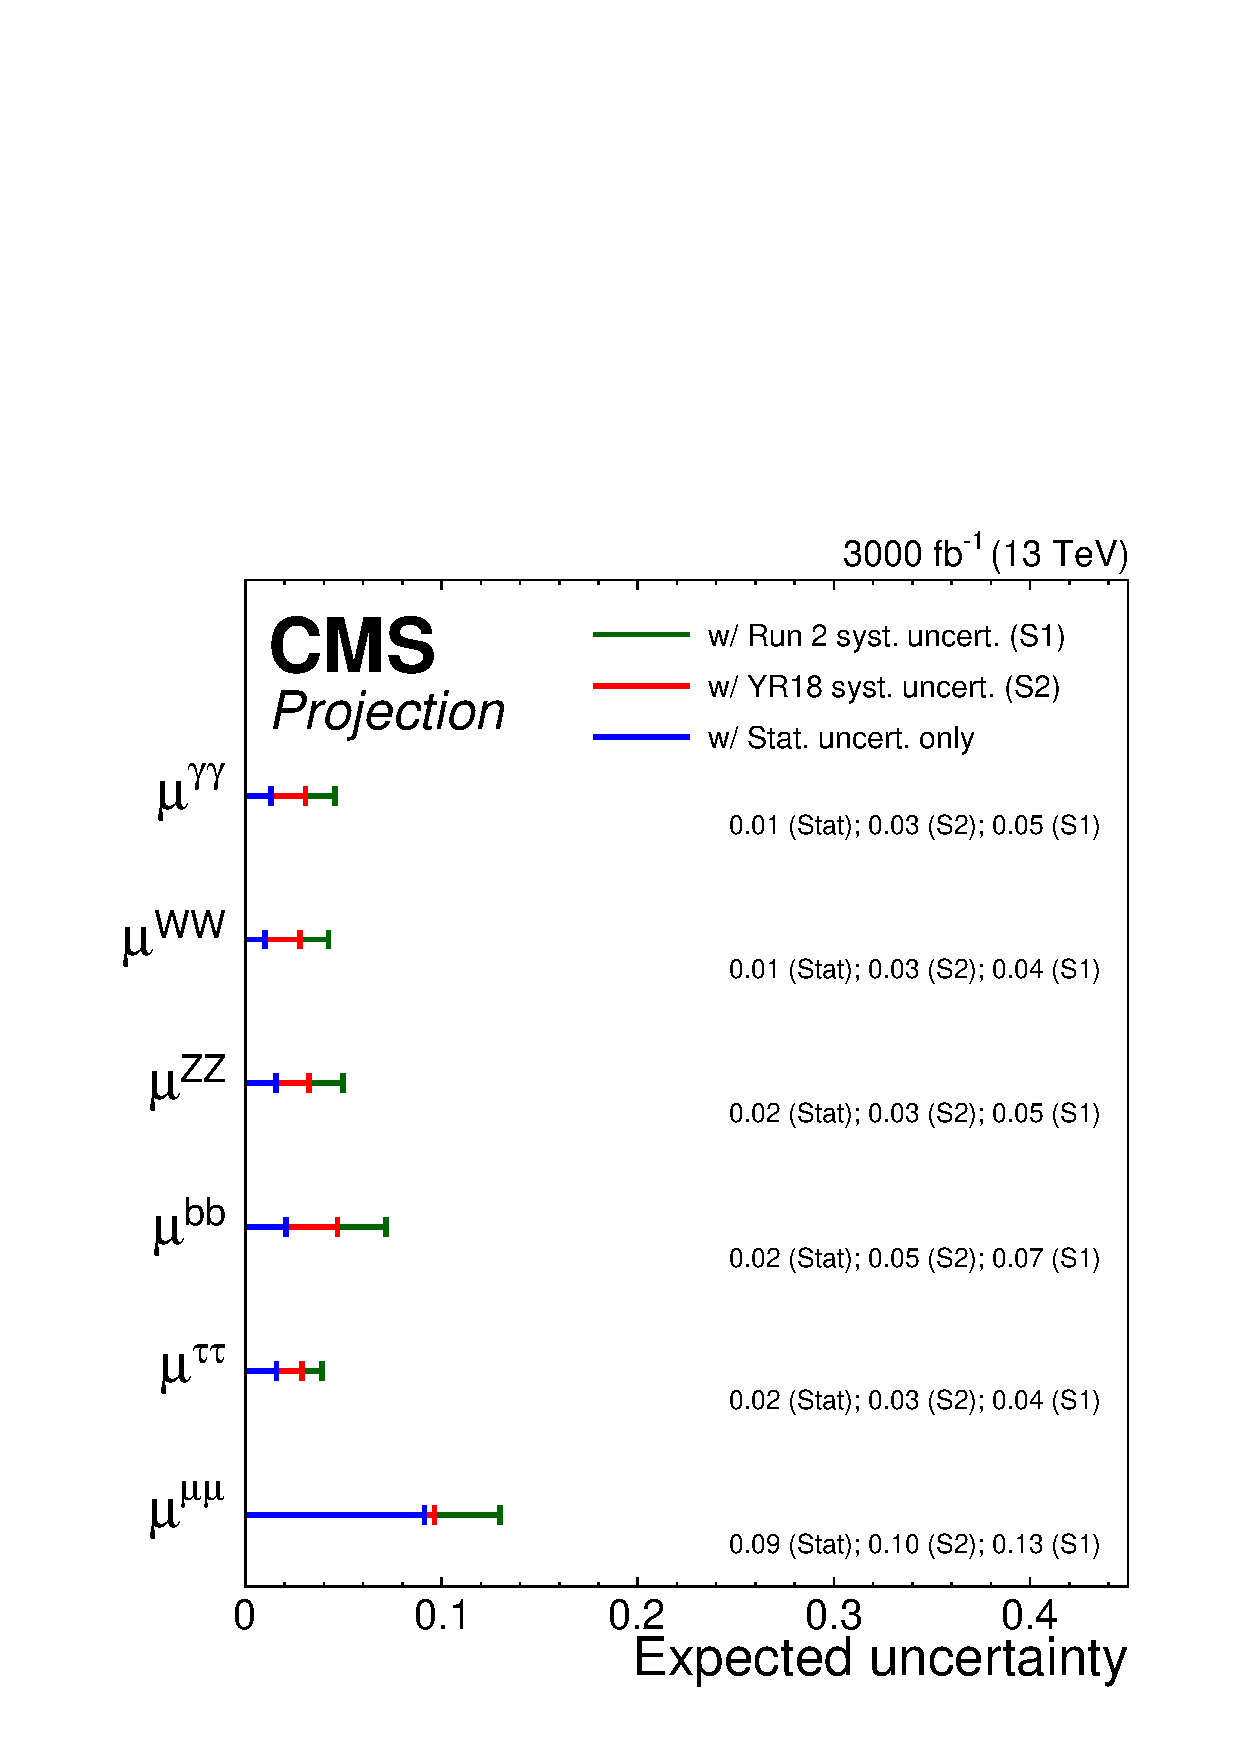
\includegraphics[width=0.6\textwidth]{\main/section2/plots/comb/summary_A1_5D_3000.pdf}%
\caption{Summary plot showing the total expected $\pm 1\sigma$ uncertainties in S1 (with Run~2 systematic uncertainties~\cite{Sirunyan:2018koj}) and S2 (with YR18 systematic uncertainties) on the per-decay-mode signal strength parameters. The statistical-only component of the uncertainty is also shown.}
\label{fig:summary_A1_5D}
\end{figure}


\begin{table}[hbtp]
\centering
\caption{The expected $\pm 1\sigma$ uncertainties, expressed as percentages, on the per-decay-mode signal strength parameters. Values are given for both S1 (with Run~2 systematic uncertainties~\cite{Sirunyan:2018koj}) and S2 (with YR18 systematic uncertainties). The total uncertainty is decomposed into four components: statistical (Stat), signal theory (SigTh), background theory (BkgTh) and experimental (Exp).}
\begin{tabular}{@{} l c c@{\hskip 0.15in} c c c c @{}}
 \hline
  &  & \multicolumn{5}{c}{3000 $\text{fb}^{-1}$} \\
  &  & Total & Stat & SigTh & BkgTh & Exp \\
 \hline
\multirow{2}{*}{$\mu^{\gamma \gamma }$} & S1  & 4.6& 1.3 & 3.5 & 0.3 & 2.6  \\[1pt]
                        & S2  & 3.1& 1.3 & 2.1 & 0.3 & 1.7  \\[4pt]
\multirow{2}{*}{$\mu^{\mathrm{WW}}$} & S1  & 4.2& 1.0 & 3.7 & 1.0 & 1.4  \\[1pt]
                        & S2  & 2.8& 1.0 & 2.2 & 0.9 & 1.1  \\[4pt]
\multirow{2}{*}{$\mu^{\mathrm{ZZ}}$} & S1  & 5.0& 1.6 & 3.5 & 1.9 & 2.5  \\[1pt]
                        & S2  & 3.3& 1.6 & 2.1 & 0.7 & 1.7  \\[4pt]
\multirow{2}{*}{$\mu^{\mathrm{bb}}$} & S1  & 7.2& 2.1 & 5.4 & 3.6 & 2.3  \\[1pt]
                        & S2  & 4.7& 2.1 & 2.5 & 2.9 & 1.7  \\[4pt]
\multirow{2}{*}{$\mu^{\tau \tau }$} & S1  & 3.9& 1.6 & 2.6 & 1.5 & 1.9  \\[1pt]
                        & S2  & 2.9& 1.6 & 1.8 & 0.6 & 1.4  \\[4pt]
\multirow{2}{*}{$\mu^{\mu\mu}$} & S1  & 13.0& 9.1 & 5.2 & 0.8 & 7.6  \\[1pt]
                        & S2  & 9.6& 9.1 & 2.6 & 0.8 & 1.7  \\[4pt]
\hline
\end{tabular}
\label{tab:summary_A1_5D}
\vspace{0.5cm}
\end{table}

Another important aspect of the projected measurements is how the correlations between the measured parameters are expected to evolve. Correlations arise when analysis channels are sensitive to more than one production or decay mode and the chosen fit observables do not fully distinguish between these. In addition, correlations may arise when the same systematic uncertainties apply to multiple production or decay modes. Figure~\ref{fig:corr_A1_5D} shows the correlation coefficients between the signal strength parameters in S2. The correlations range up to $+0.44$, and are largest between modes where the sensitivity is dominated by gluon-fusion production. This reflects the impact of the theory uncertainties affecting the SM prediction of the gluon-fusion production rate.

\begin{figure}[hbtp]
\centering
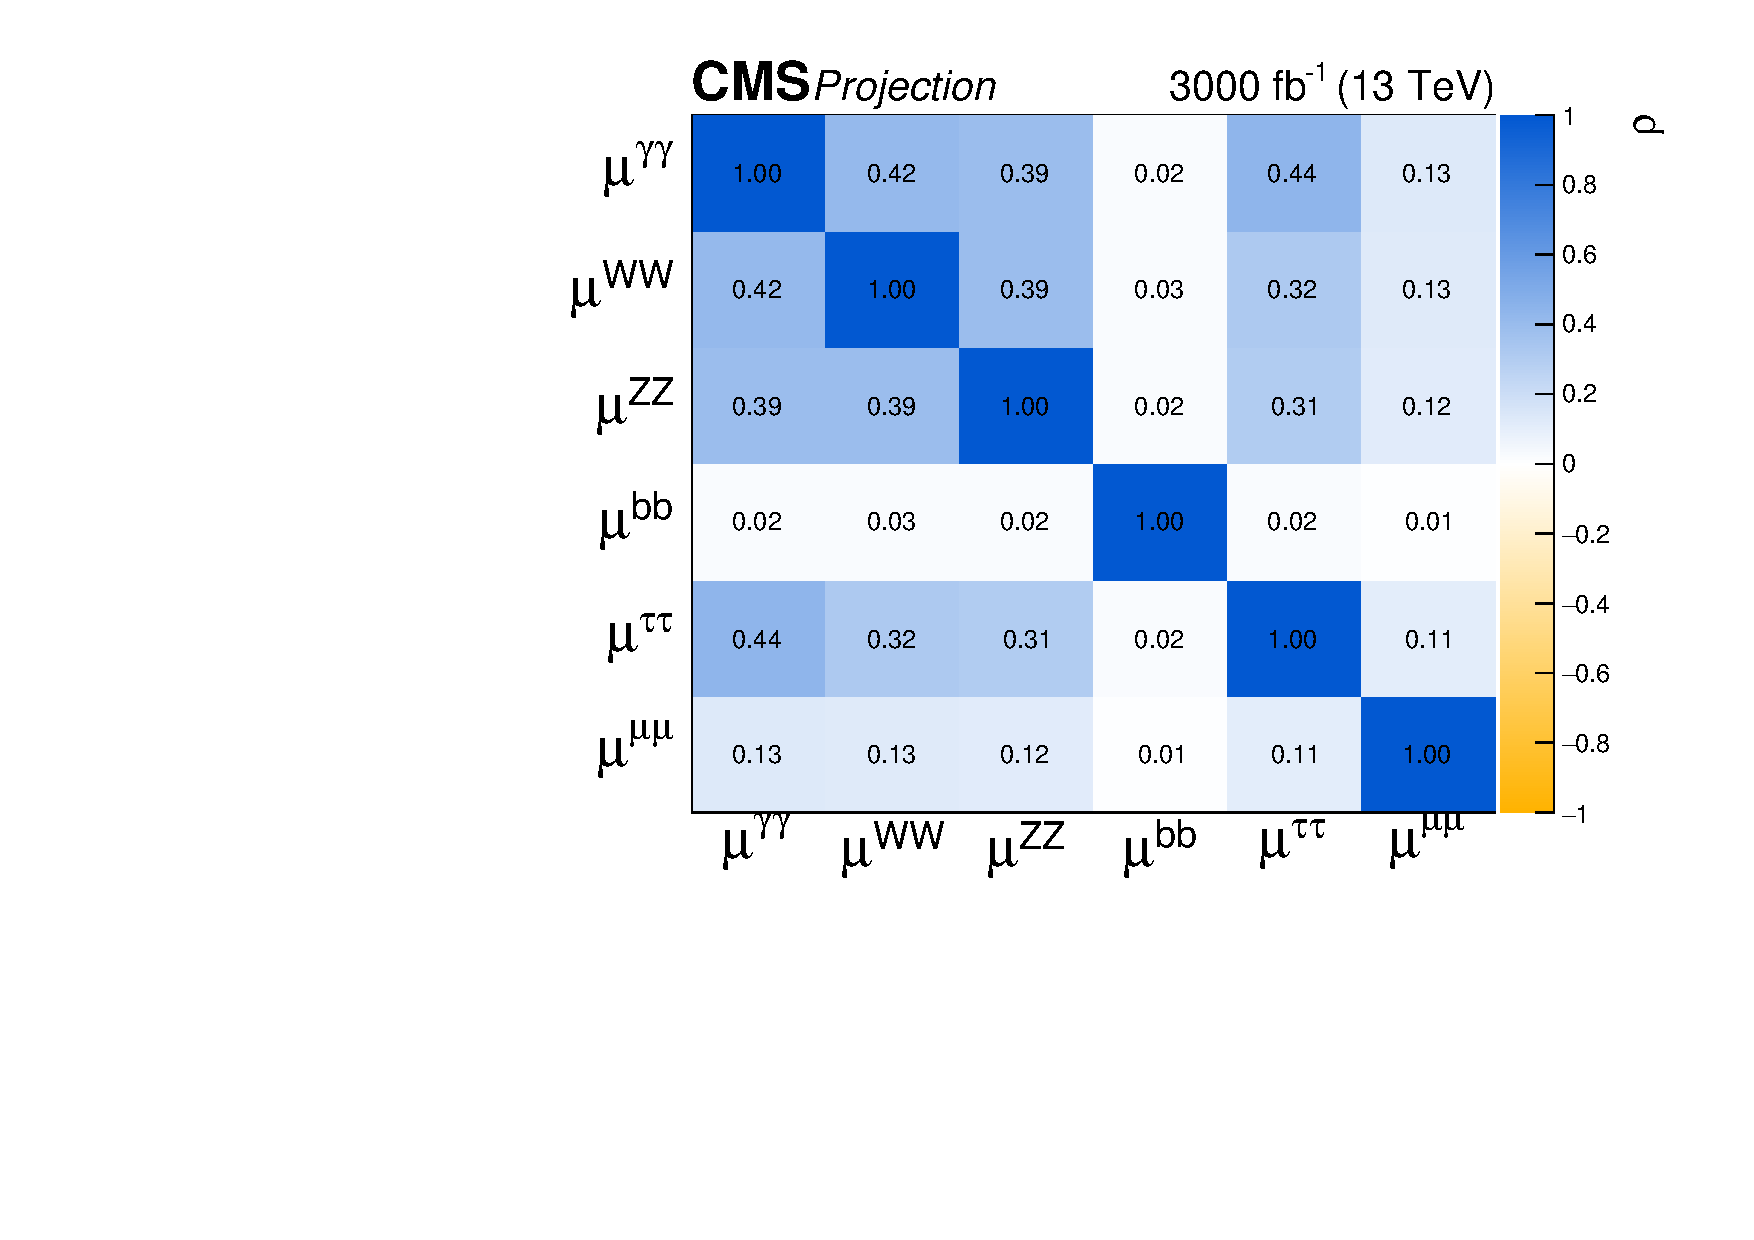
\includegraphics[width=0.6\textwidth]{\main/section2/plots/comb/correlations_A1_5D_S2_3000.pdf}%
\caption{Correlation coefficients ($\rho$) between parameters in the signal strength per-decay-mode parametrisation for S2 (with YR18 systematic uncertainties).}
\label{fig:corr_A1_5D}
\end{figure}

\subsubsection{Signal strength per-production mode}
The expected $\pm 1\sigma$ uncertainties on the per-production-mode signal strength parameters in S1 and S2 are summarised in Figure~\ref{fig:summary_A1_5P} with numerical values given in Table~\ref{tab:summary_A1_5P}. In S1 the signal theory is the main contribution for all modes except $\wh$ which remains limited by statistics. In S2 $\mu_{\vbf}$ and $\mu_{\wh}$ are also statistically limited.


\begin{figure}[hbtp]
\centering
% \includegraphics[width=0.48\textwidth]{\main/section2/plots/comb/summary_A1_5P_300.pdf}%
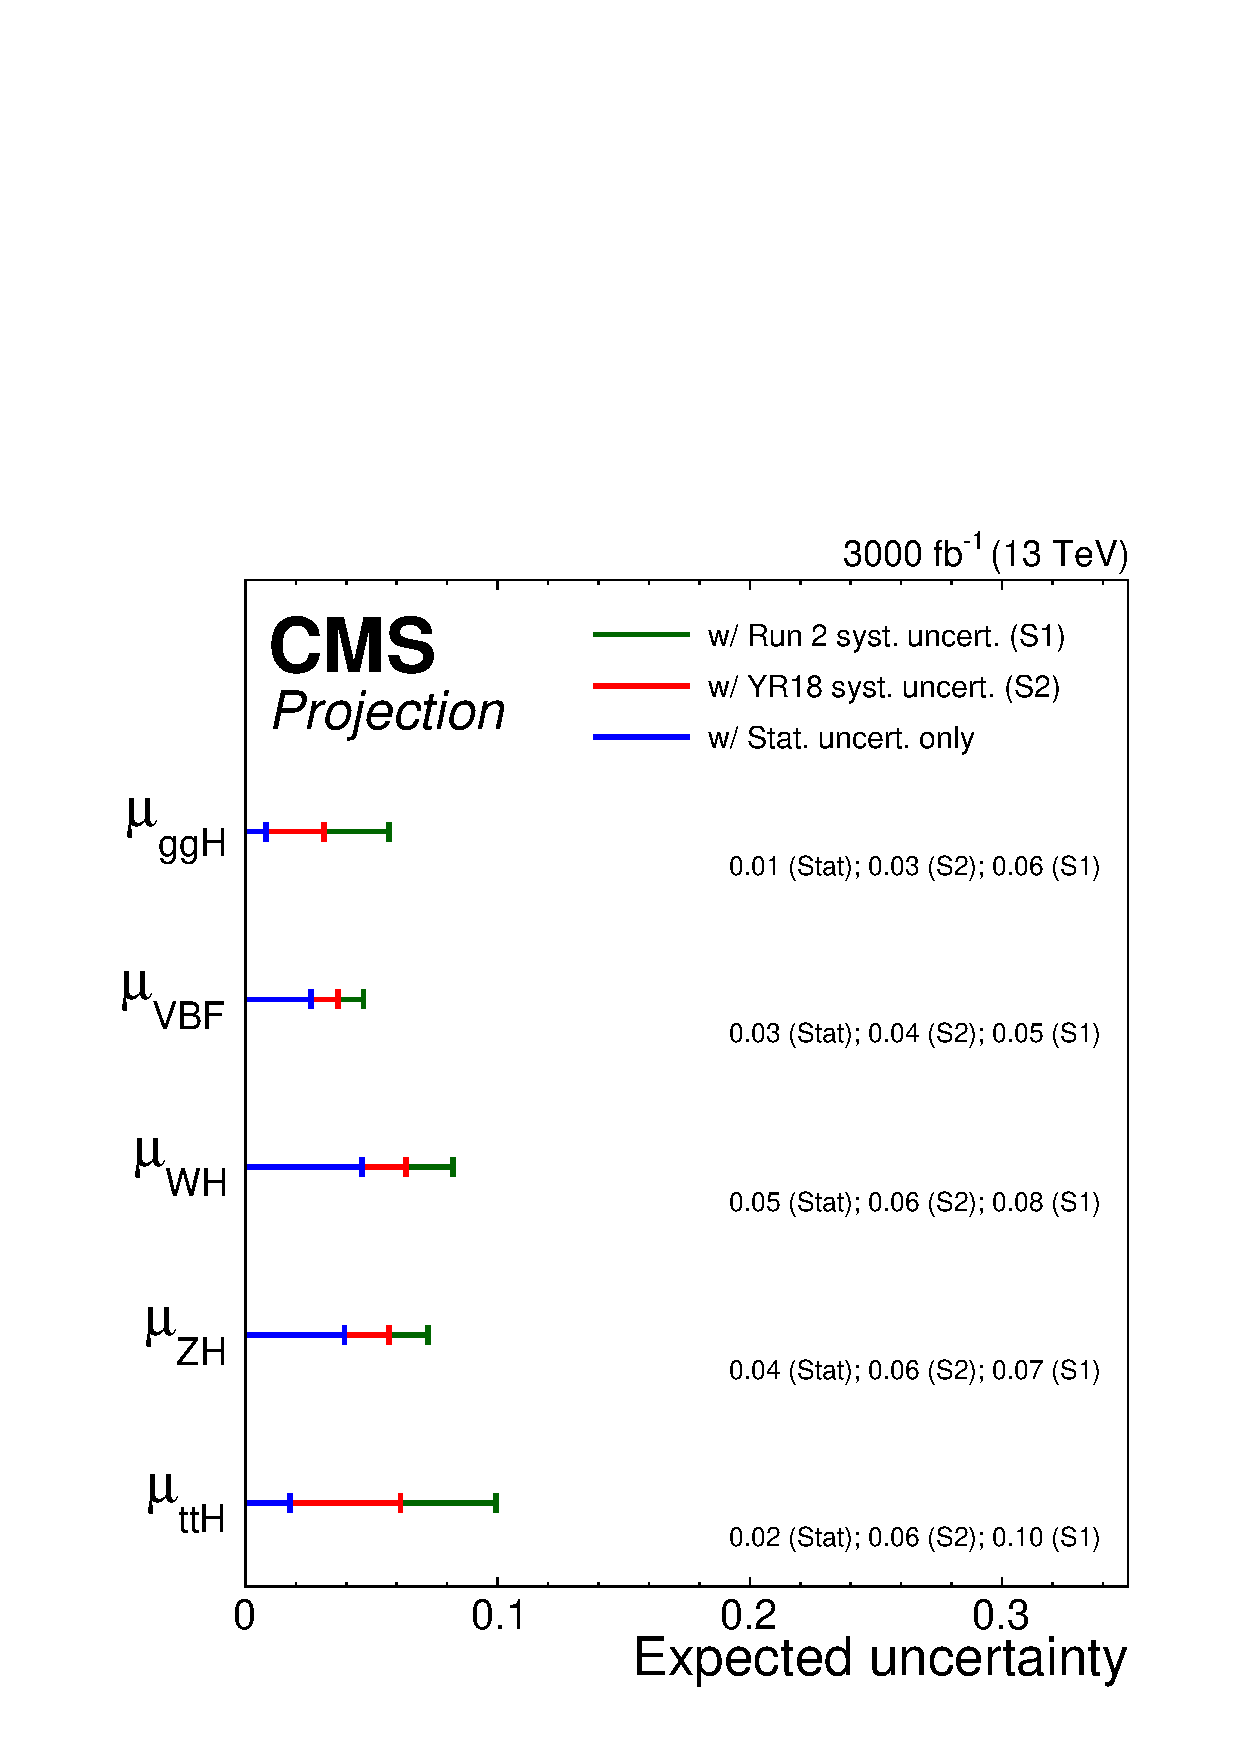
\includegraphics[width=0.6\textwidth]{\main/section2/plots/comb/summary_A1_5P_3000.pdf}%
\caption{Summary plot showing the total expected $\pm 1\sigma$ uncertainties in S1 (with Run~2 systematic uncertainties~\cite{Sirunyan:2018koj}) and S2 (with YR18 systematic uncertainties) on the per-production-mode signal strength parameters. The statistical-only component of the uncertainty is also shown.}
\label{fig:summary_A1_5P}
\end{figure}


\begin{table}[hbtp]
\centering
\caption{The expected $\pm 1\sigma$ uncertainties, expressed as percentages, on the per-production-mode signal strength parameters. Values are given for both S1 (with Run~2 systematic uncertainties~\cite{Sirunyan:2018koj}) and S2 (with YR18 systematic uncertainties). The total uncertainty is decomposed into four components: statistical (Stat), signal theory (SigTh), background theory (BkgTh) and experimental (Exp).}
\begin{tabular}{@{} l c c@{\hskip 0.15in} c c c c @{}}
 \hline
  &  & \multicolumn{5}{c}{3000 $\text{fb}^{-1}$} \\
  &  & Total & Stat & SigTh & BkgTh & Exp \\
 \hline
\multirow{2}{*}{$\mu_{\mathrm{ggH}}$} & S1  & 5.7& 0.8 & 5.4 & 0.9 & 1.2  \\[1pt]
                        & S2  & 3.1& 0.8 & 2.8 & 0.6 & 0.9  \\[4pt]
\multirow{2}{*}{$\mu_{\mathrm{VBF}}$} & S1  & 4.7& 2.6 & 3.0 & 1.3 & 2.1  \\[1pt]
                        & S2  & 3.7& 2.6 & 2.1 & 0.3 & 1.6  \\[4pt]
\multirow{2}{*}{$\mu_{\mathrm{WH}}$} & S1  & 8.2& 4.6 & 2.9 & 3.3 & 5.2  \\[1pt]
                        & S2  & 6.4& 4.6 & 1.4 & 2.7 & 3.2  \\[4pt]
\multirow{2}{*}{$\mu_{\mathrm{ZH}}$} & S1  & 7.2& 3.9 & 5.1 & 2.5 & 2.1  \\[1pt]
                        & S2  & 5.7& 3.9 & 3.0 & 2.3 & 1.7  \\[4pt]
\multirow{2}{*}{$\mu_{\mathrm{ttH}}$} & S1  & 9.9& 1.8 & 8.3 & 4.1 & 3.1  \\[1pt]
                        & S2  & 6.2& 1.8 & 4.2 & 3.4 & 2.4  \\[4pt]
\hline
\end{tabular}
\label{tab:summary_A1_5P}
\vspace{0.5cm}
\end{table}

Figure~\ref{fig:corr_A1_5P} shows the correlation coefficients between the signal strength parameters in S2. The correlations in this case are small compared to the per-decay measurements since production modes are generally well-isolated by independent analysis categories and the main theoretical uncertainties on the SM signal expectation are uncorrelated.

\begin{figure}[hbtp]
\centering
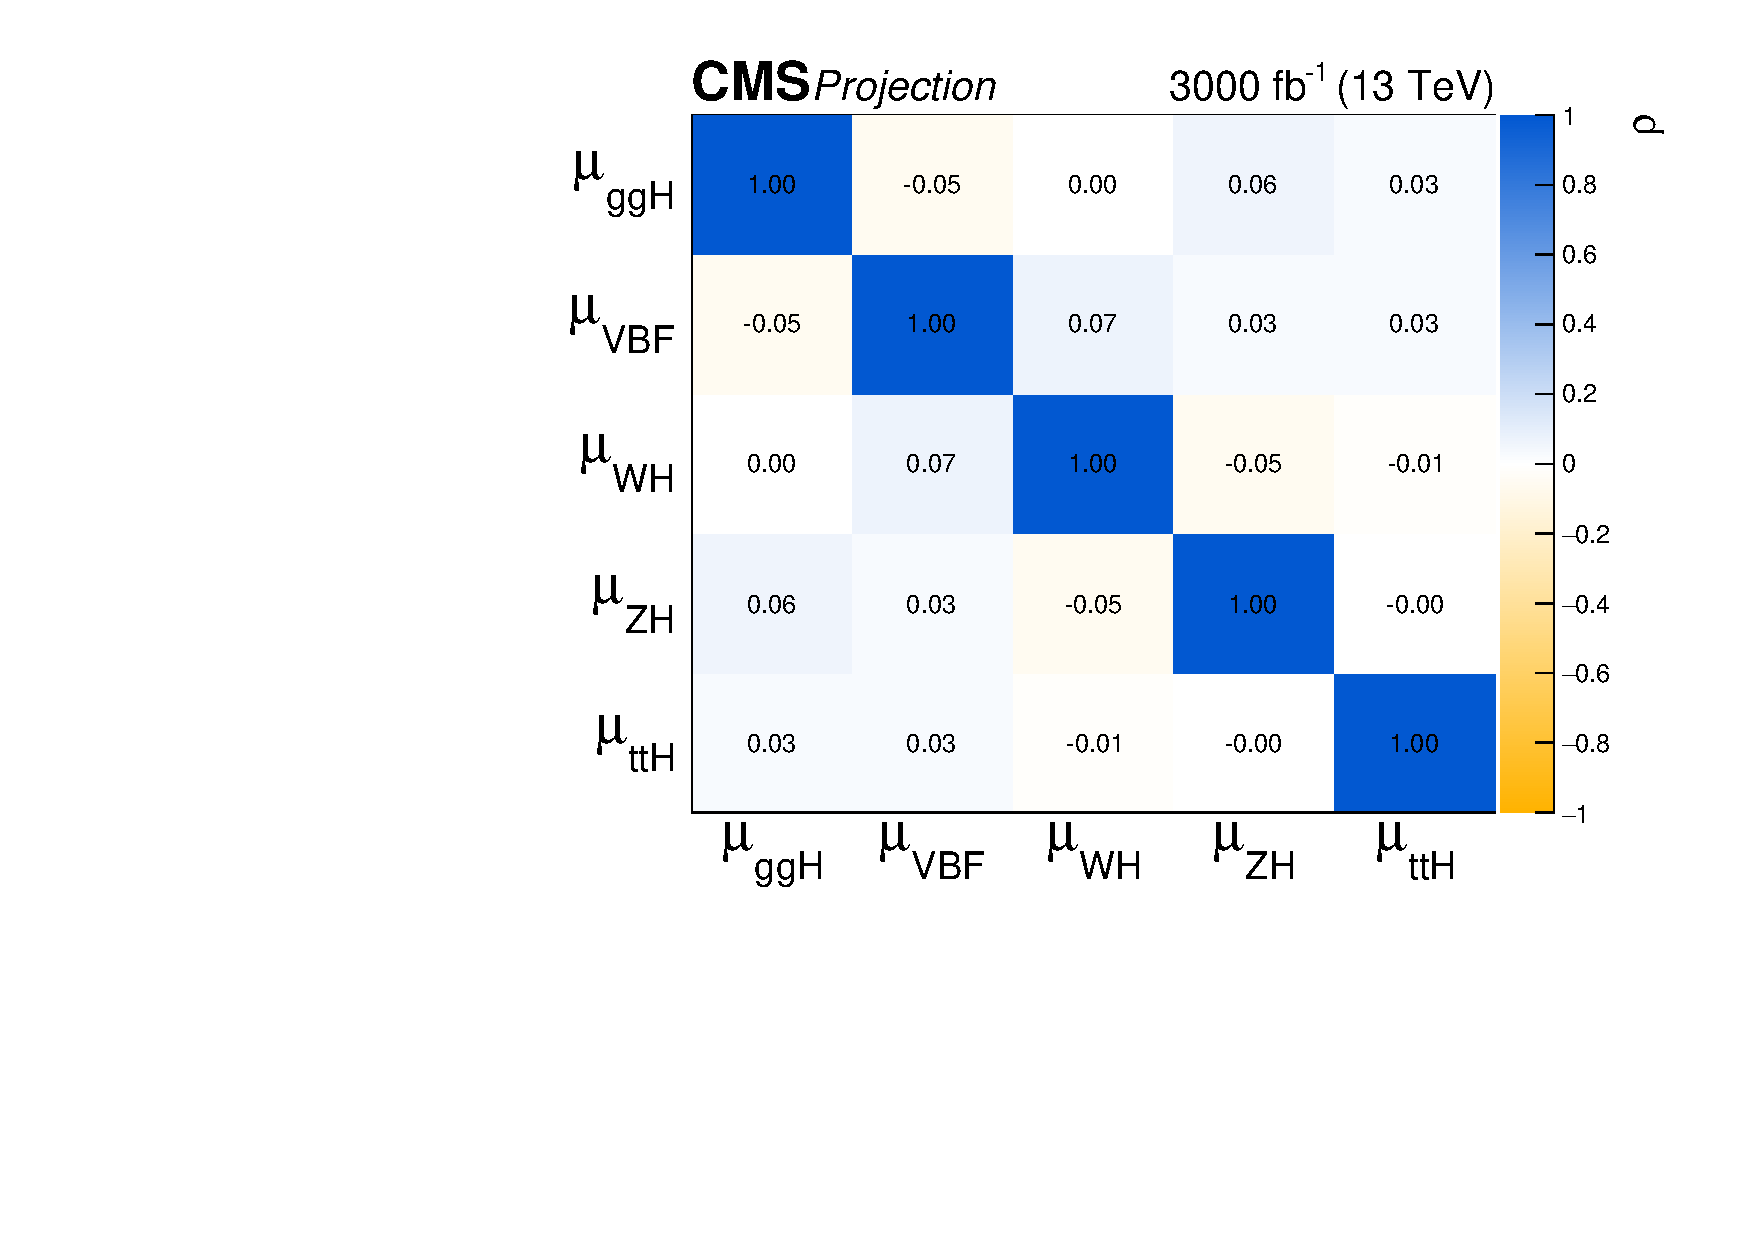
\includegraphics[width=0.6\textwidth]{\main/section2/plots/comb/correlations_A1_5P_S2_3000.pdf}%
\caption{Correlation coefficients ($\rho$) between parameters in the signal strength per-production-mode parametrisation for S2 (with YR18 systematic uncertainties) at $300\fbinv$ (left) and $3000\fbinv$ (right).}
\label{fig:corr_A1_5P}
\end{figure}
